\documentclass[14pt,a4paper]{extarticle}
\usepackage{amsmath}
\usepackage{amsfonts}
\usepackage{amssymb}
\usepackage{amsthm}
\usepackage{afterpage}
\usepackage{braket}
\usepackage{enumitem}
\usepackage{fancyhdr}
\usepackage{graphicx}
\usepackage{setspace}
\usepackage{subcaption}

\title{What is the pricing strategy of Big Mountain Resort?}
\author{Noravee Kanchanavatee}

\begin{document}
	\maketitle
	\section*{Findings}
	\begin{itemize}
		\item Ticket price without investment: \textbf{\$86}
		\item Ticket price with investment: \textbf{\$88}
	\end{itemize}
	\begin{figure}
		\centering
		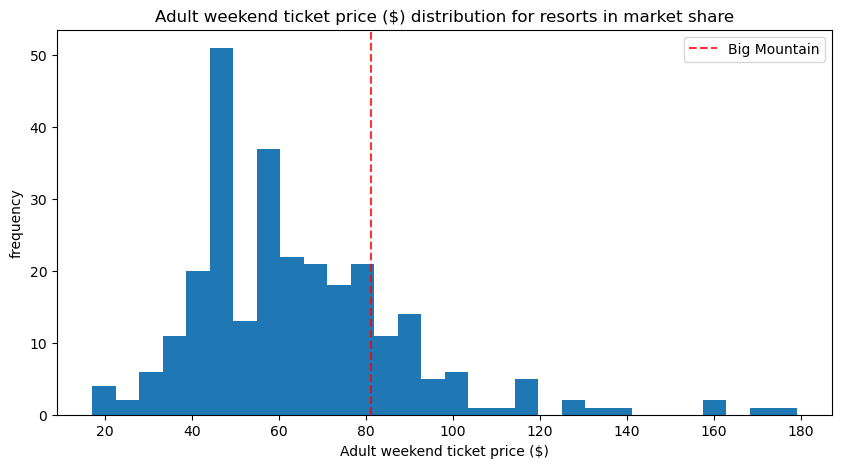
\includegraphics[width=0.7\textwidth]{Price}
		\caption{Distribution of ticket price for ski resorts in the US}
		\label{fig1}
	\end{figure}
	Big Mountain Resort, a ski resort located in Montana, offers spectacular views of Glacier National Park and Flathead National Forest. Every year about 350,000 people ski or snowboard at Big Mountain with average stay of 5 days. The current ticket price is \$81 per, however, Big Mountain Resort has recently installed an additional chair lift to help increase the distribution of visitors across the mountain, which increases their operating costs by \$1,540,000. This makes the break even price \$82, assuming the same amount of tickets sold.
	
	Our model identifies key assets of the resort as the following:
	\begin{itemize}
		\item Vertical drop
		\item Area covered by snow making machines
		\item Number of chair lifts
		\item Number of fast four person chairs
	\end{itemize}
	Taking this information into account, the current price is too low. These facilities rank at the 90th percentile or above among all ski resort in the country while the ticket price is only at the 80th percentile as can be seen in Figure \ref{fig1}. To reflect the quality of the facilities, the price would be in the range of \$86 to \$106. Conversly, the current price is already at the top of ski resorts in Montana. Thus, the most reasonable price is \$86.  
	
	The following adjustment has been proposed to hopefully either cut costs without undermining the ticket price or support an even higher ticket price.
	\begin{enumerate}
		\item Permanently closing down up to 10 of the least used runs \\[0.5cm]
		According to our model, the result of closing down trails can be seen in the Table \ref{table1}.
		\begin{table}
			\centering
			\renewcommand{\arraystretch}{1.2}
		\begin{tabular}{|c|c|c|}
			\hline
			Run closed & Price decrease & Ticket prices \\
			\hline
			1 & \$0 & \$86.00\\
			2 & \$0.41 & \$85.59\\
			3-5 & \$0.67 & \$85.33 \\
			6-8 & \$1.26 & \$84.74 \\
			9 & \$1.71 & \$84.29 \\
			10 & \$1.81 & \$84.19 \\
			\hline
		\end{tabular}
		\caption{Number of closed runs, price decrease, and ticket prices}
		\label{table1}
		\end{table}
		The model says closing one run makes no difference. Closing 2 and 3 successively reduces support for ticket price. If Big Mountain closes down 3 runs, it seems they may as well close down 4 or 5 as there's no further loss in ticket price. Increasing the closures down to 6 or more leads to a large drop.
		\item Increase the vertical drop by adding a run to a point 150 feet lower down but requiring the installation of an additional chair lift \\[0.5cm]
		This scenario increases the operating cost due to the chair installation by \$1.5M, but supports the increase in ticket price for \$2.
		\item Same as number 2, but adding 2 acres of snow making cover area\\[0.5cm]
		Consider the Resort already has roughly 600 acre of snow making area. Increase it by 2 acre have no positive impact on the price, and only add up the operating cost.
		\item Increase the longest run by 0.2 mile to boast 3.5 miles length, requiring an additional snow making coverage of 4 acres \\[0.5cm]
		The distance of the longest run is not one of the key features in our model, and 4 acres is still very small compared to 600 acres. This change has no effect on price.
	\end{enumerate}
	
	\section*{Summary}
		Current facilities of the resort can support \$86 ticket price. Enhancing the assets by adding a run which increase the vertical drop and add another chair will support \$2 price increase. Cost cutting can be done by closing down the least used run without any impact on the price.
\end{document}